%\documentclass{beamer}
\documentclass[usenames,dvipsnames]{beamer}
\usepackage{tikz}

\usetheme{Frankfurt}

\title{MATH 4802\\Presentation 3, Group 4}
\author{Lixin Zheng, Alexander Divoux, Andrew Wittenmyer, Ethan Curtiss, Jaeyoung Beck, Lance Lampert, Neil Patram, Pavan Mayinampati, Sean Eva, Vasisht Ganesh, Walter Kirkland}
\date{November 1, 2021}

\begin{document}

\maketitle

\begin{frame}
	\frametitle{Problem: 2009 A1}

	Let $f$ be a real-valued function on the plane such that for every square $ABCD$ in the plane, $f(A)+f(B)+f(C)+f(D)=0$. Does it follow that $f(P)=0$ for all points $P$ in the plane?
\end{frame}

\begin{frame}
    \frametitle{Solution}
        \centering
            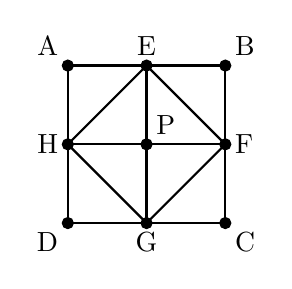
\begin{tikzpicture}
            %\draw[step=0.5cm, gray, very thin] (0, 0) grid (4, 4);
        
            \draw[thick] (1, 1) rectangle (3, 3); %ABCD
            \draw[thick] (1, 2) -> (2, 3) -> (3, 2) -> (2,1) -> (1,2); %EFGH
            \draw[thick] (1, 2) -> (3, 2); %EG
            \draw[thick] (2, 1) -> (2, 3); %HF
            
            % Letters
            \node [above left] at (1, 3) {A};
            \node [above right] at (3, 3) {B};
            \node [below left] at (1, 1) {D};
            \node [below right] at (3, 1) {C};

            \node [above right] at (2, 2) {P};
            
            \node [above] at (2, 3) {E};
            \node [right] at (3, 2) {F};
            \node [left] at (1, 2) {H};
            \node [below] at (2, 1) {G};
            
            % Points
            \filldraw (2, 2) circle (2pt);
            \filldraw (1, 3) circle (2pt);
            \filldraw (3, 3) circle (2pt);
            \filldraw (1, 1) circle (2pt);
            \filldraw (3, 1) circle (2pt);
            
            \filldraw (2, 3) circle (2pt);
            \filldraw (3, 2) circle (2pt);
            \filldraw (1, 2) circle (2pt);
            \filldraw (2, 1) circle (2pt);
            
        \end{tikzpicture}
        
        \bigskip
    
    
    
    \begin{columns}
        \column{0.8\textwidth}
        Let $P$ be any point in the plane. Define an arbitrary square $ABCD$ in the plane with center $P$ and corners labeled $A, B, C, D$. Let the midpoints of $AB, BC, CD, DA$ be $E, F, G, H$ (respectively).
    \end{columns}
\end{frame}

\begin{frame}
    \frametitle{Solution}
    
    \centering
        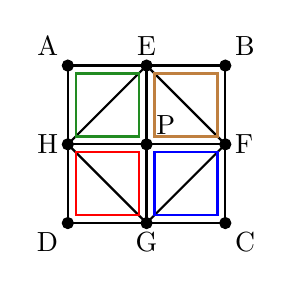
\begin{tikzpicture}
            %\draw[step=0.5cm, gray, very thin] (0, 0) grid (4, 4);
        
        
            \draw[thick] (1, 1) rectangle (3, 3); %ABCD
            \draw[thick] (1, 2) -> (2, 3) -> (3, 2) -> (2,1) -> (1,2); %EFGH
            \draw[thick] (1, 2) -> (3, 2); %EG
            \draw[thick] (2, 1) -> (2, 3); %HF
            
            \draw[thick, red] (1.1, 1.1) rectangle (1.9, 1.9); %HPGD
            \draw[thick, blue] (2.1, 1.1) rectangle (2.9, 1.9); %PFGC
            \draw[thick, ForestGreen] (1.1, 2.1) rectangle (1.9, 2.9); %AEPH
            \draw[thick, brown] (2.1, 2.1) rectangle (2.9, 2.9); %EBFP
            
            
            % Letters
            \node [above left] at (1, 3) {A};
            \node [above right] at (3, 3) {B};
            \node [below left] at (1, 1) {D};
            \node [below right] at (3, 1) {C};

            \node [above right] at (2, 2) {P};
            
            \node [above] at (2, 3) {E};
            \node [right] at (3, 2) {F};
            \node [left] at (1, 2) {H};
            \node [below] at (2, 1) {G};
            
            % Points
            \filldraw (2, 2) circle (2pt);
            \filldraw (1, 3) circle (2pt);
            \filldraw (3, 3) circle (2pt);
            \filldraw (1, 1) circle (2pt);
            \filldraw (3, 1) circle (2pt);
            
            \filldraw (2, 3) circle (2pt);
            \filldraw (3, 2) circle (2pt);
            \filldraw (1, 2) circle (2pt);
            \filldraw (2, 1) circle (2pt);
            
        \end{tikzpicture}
    
    
    
    \begin{columns}
    
        \column{0.8\textwidth}
        We note $AEPH, EBFP, PFCG, HPGD$ are all squares, so 
        {\scriptsize
        \begin{alignat*}{9}
            &{\color{ForestGreen}f(A)} &&&&+{\color{ForestGreen}f(E)} &&&+{\color{ForestGreen}f(H)} &+{\color{ForestGreen}f(P)}&=0\\
            &&{\color{brown}f(B)}&&&+{\color{brown}f(E)}&+{\color{brown}f(F)} &&&+{\color{brown}f(P)}&=0\\
            &&&{\color{blue}f(C)}&&&+{\color{blue}f(F)}&+{\color{blue}f(G)} &&+{\color{blue}f(P)}&=0\\
            +&&&&{\color{red}f(D)}&&&+{\color{red}f(G)}&+{\color{red}f(H)} &+{\color{red}f(P)}&=0\\
            \hline\\
            (&{\color{Magenta}f(A)}+&{\color{Magenta}f(B)}+&{\color{Magenta}f(C)}+&{\color{Magenta}f(D)})\\
            &&&&&+2({\color{orange}f(E)}&+{\color{orange}f(F)}&+{\color{orange}f(G)}&+{\color{orange}f(H)})\\
            &&&&&&&&&+4f(P)&=0
        \end{alignat*}}
        \end{columns}
\end{frame}


\begin{frame}
    \frametitle{Solution}
        \centering
        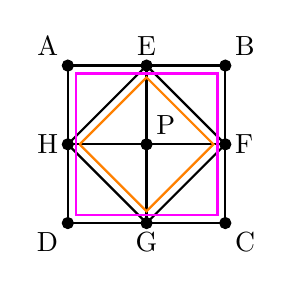
\begin{tikzpicture}
            %\draw[step=0.5cm, gray, very thin] (0, 0) grid (4, 4);
        
        
            \draw[thick] (1, 1) rectangle (3, 3); %ABCD
            \draw[thick] (1, 2) -> (2, 3) -> (3, 2) -> (2,1) -> (1,2); %EFGH
            \draw[thick] (1, 2) -> (3, 2); %EG
            \draw[thick] (2, 1) -> (2, 3); %HF
            
            %\draw[thick, red] (1.1, 1.1) rectangle (1.9, 1.9); %HPGD
            %\draw[thick, blue] (2.1, 1.1) rectangle (2.9, 1.9); %PFGC
            %\draw[thick, ForestGreen] (1.1, 2.1) rectangle (1.9, 2.9); %AEPH
            %\draw[thick, brown] (2.1, 2.1) rectangle (2.9, 2.9); %EBFP
            
            \draw[thick, Magenta] (1.1, 1.1) rectangle (2.9, 2.9); %ABCD
            \draw[thick, orange] (1.15, 2) -> (2, 2.85) -> (2.85, 2) -> (2,1.15) -> (1.15,2);
            
            % Letters
            \node [above left] at (1, 3) {A};
            \node [above right] at (3, 3) {B};
            \node [below left] at (1, 1) {D};
            \node [below right] at (3, 1) {C};

            \node [above right] at (2, 2) {P};
            
            \node [above] at (2, 3) {E};
            \node [right] at (3, 2) {F};
            \node [left] at (1, 2) {H};
            \node [below] at (2, 1) {G};
            
            % Points
            \filldraw (2, 2) circle (2pt);
            \filldraw (1, 3) circle (2pt);
            \filldraw (3, 3) circle (2pt);
            \filldraw (1, 1) circle (2pt);
            \filldraw (3, 1) circle (2pt);
            
            \filldraw (2, 3) circle (2pt);
            \filldraw (3, 2) circle (2pt);
            \filldraw (1, 2) circle (2pt);
            \filldraw (2, 1) circle (2pt);
            
        \end{tikzpicture}
        
        
            \begin{columns}
        \column{0.8\textwidth}
        
        {\scriptsize
        \begin{alignat*}{9}
            (&{\color{Magenta}f(A)}+&{\color{Magenta}f(B)}+&{\color{Magenta}f(C)}+&{\color{Magenta}f(D)})\\
            &&&&&+2({\color{orange}f(E)}&+{\color{orange}f(F)}&+{\color{orange}f(G)}&+{\color{orange}f(H)})\\
            &&&&&&&&&+4f(P)&=0
        \end{alignat*}}
        We know that $ABCD$ and $EFGH$ are both squares, so the pink and orange sums are both 0. This leaves us with $4f(P) = 0 \implies f(P) = 0$. As $P$ was chosen arbitrarily we conclude $f(P) = 0$ for all points $P$ in the plane.
        
        \end{columns}
\end{frame}



\end{document}